\documentclass[a4paper,titlepage,10pt]{article}
\usepackage{spreadtab}
\usepackage{url}
\usepackage{siunitx}
\usepackage{graphicx}
\usepackage{placeins}

\usepackage{spreadtab}
\usepackage{spreadtab}
\usepackage{url}
\usepackage{siunitx}
\usepackage{graphicx}
\usepackage{placeins}

\usepackage{spreadtab}
\usepackage{url}
\usepackage{siunitx}
\usepackage{graphicx}
\usepackage{placeins}
\usepackage{amsmath}

\usepackage{spreadtab}
\usepackage{graphicx}
\usepackage{placeins}

\input{scope_conclusion_preamble.tex}
\usepackage{spreadtab}
\usepackage{url}
\usepackage{siunitx}
\usepackage{graphicx}
\usepackage{placeins}
\usepackage{amsmath}

\usepackage{verbatim}
\usepackage{geometry}
\geometry{left=20mm}

\usepackage{standalone}
\usepackage{geometry}
\geometry{left=20mm}
\begin{document}

\begin{titlepage}
	\centering
	\vspace{2.5cm}
	{\huge Experiment 1 \par}
	{\LARGE Introduction and Equipment Operations \par}
	\vspace{1cm}
	{\Large EECS 170A - Lab Bench \#1 \par}
	{\Large \today \par}
	\vspace{1cm}
	{\large Roman Parise (59611417) \par}
	{\large Krishan Solanki (38154673) \par}
	{\large Jason Wang (42873192) \par}
	\vspace{1cm}
\end{titlepage}

\clearpage

\section{Procedure}
\subsection{Voltmeter Impedance}
%For the Electronics Lab course, the multimeter model that is being used is the 34405A. This multimeter helps measure features such as either true RMS AC or DC voltage and as well as true RMS AC or DC current. The range of the voltage on the multimeter goes from 10mV to 1000V, while the range for the current goes from 10mA to 10A \cite{34405A:3}. The input impedance of the multimeter is around 1M\si{\ohm} +/- 2\% for AC voltage while the input resistance for DC voltage is listed around 10M\si{\ohm} +/-2\%\cite{34405A:6}. The circuit in this lab is a simple series circuit, therefore the voltmeter acts as a voltage divider.\\
\\

\begin{figure}[h!]
\centering
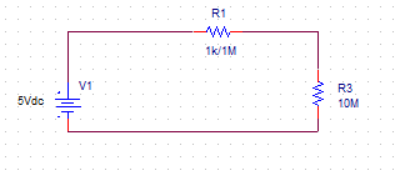
\includegraphics{voltmeterfinal.PNG}
\caption{Voltmeter Circuit Model}
\label{fig:Voltmeter_Pic}
\end{figure}

\begin{equation}
	\label{eq:vdvm}
	V_{DVM} = V_{Source}(\frac{R_{DVM}}{R_{DVM} + R}) 
\end{equation}

For the circuit with the voltmeter, students will measure the voltage across a voltmeter on a circuit using resistors of value 1kΩ and 1MΩ simultaneously. After measuring the voltage, equation \ref{eq:vdvm} can be used to find the impedance of the DVM from the voltmeter's voltage, the source's voltage, and the resistance R. To finish off this part of the experiment, the measured voltmeter impedance is compared to the manufacturer's results. 

For the Electronics Lab course, the multimeter model that is being used is the 34405A. This multimeter helps measure features such as either true RMS AC or DC voltage and as well as true RMS AC or DC current. The range of the voltage on the multimeter goes from 10mV to 1000V, while the range for the current goes from 10mA to 10A. The input impedance of the multimeter is around 1M\si{\ohm} +/- 2\% for AC voltage while the input resistance for DC voltage is listed around 10M\si{\ohm} +/-2\% [\ref{itm:34405A}]. The circuit in this lab is a simple series circuit, therefore the voltmeter acts as a voltage divider.\\
\\

\begin{figure}[h!]
\centering
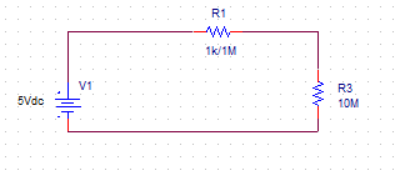
\includegraphics{voltmeterfinal.PNG}
\caption{Voltmeter Circuit Model}
\label{fig:Voltmeter_Pic}
\end{figure}

\begin{equation}
	\label{eq:vdvm}
	V_{DVM} = V_{Source}(\frac{R_{DVM}}{R_{DVM} + R}) 
\end{equation}

For the circuit with the voltmeter, students will measure the voltage across a voltmeter on a circuit using resistors of value 1k\si{\ohm} and 1M\si{\ohm} simultaneously. After measuring the voltage, equation (\ref{eq:vdvm}) can be used to find the impedance of the DVM from the voltmeter's voltage, the source's voltage, and the resistance R. To finish off this part of the experiment, the measured voltmeter impedance is compared to the manufacturer's results. 
\subsection{Oscilloscope Impedance}
%For the circuit with the oscilloscope, students will measure the voltage across the oscilloscope from a circuit using resistors of value 1MΩ and 1kΩ simultaneously while setting the frequency to 1kHz. A formula is then derived to relate the measured voltage and the battery voltage (\ref{eq:osc_ratio}), which will then be used to find the impedance of the oscilloscope by hand. The experiment will be repeated using a frequency of 1MHz.

The oscilloscope to be used in this course is the Agilent InfiniiVision DSO5034A. This oscilloscope is able to perform a variety of useful functions for this lab course including plotting input and output signal waveforms, measuring amplitudes and frequencies of periodic signals, performing Fourier Transforms for visualization of frequency peaks, etc. The oscilloscope has an input resistance rated at 1 M$\Omega$ and an input capacitance of 12 pF. It also boasts a sampling rate of 2 Giga-samples/s and a bandwidth of 300 MHz. The oscilloscope can be simply modeled as a resistor and capacitor in parallel and is connected in series with a resistor and function generator which has an internal impedance of 50 $\Omega$ and that is accounted for in the circuit model shown below: 

\begin{figure}[h!]
	\centering
	\includegraphics[scale=0.5]{"./Oscope circuit extended figure".PNG}
	\caption{Oscilloscope Testing Circuit Schematic}
	\label{fig:scope_circuit}
\end{figure}


The BNC cables used in the testing of the oscilloscope may account for some capacitance in the overall circuit. However, the effects of cables are neglected. As a result, the voltage division relation can be applied to the circuit and the following equation is derived for the voltage measured across the oscilloscope,

\begin{equation}
	\label{eq:vscope}
	V_{scope} = V_{Source}(\frac{Z_{scope}}{Z_{scope} + R + R_{Source}}) 
\end{equation}
	
where $Z_{scope}$ encompasses the input impedance modeled by $R_{scope}$ and $C_{scope}$ in parallel. The ratio between the input voltage of the oscilloscope and the voltage of the function generator would then be the following:

\begin{equation}
	\label{eq:osc_ratio}
	\frac{V_{scope}}{V_{Source}} = \frac{Z_{scope}}{Z_{scope} + R + R_{Source}} 
\end{equation}

For the circuit with the oscilloscope, students will measure the voltage across the oscilloscope from a circuit using resistors of value 1M\si{\ohm} and 1k\si{\ohm} while setting the frequency to 1kHz. Equation (\ref{eq:osc_ratio}) is used to find the ratio of the oscilloscope's measured voltage to the source voltage. The experiment will be repeated using a frequency of 1MHz.

The oscilloscope to be used in this course is the Agilent InfiniiVision DSO5034A. This oscilloscope is able to perform a variety of useful functions for this lab course including plotting input and output signal waveforms, measuring amplitudes and frequencies of periodic signals, performing Fourier Transforms for visualization of frequency peaks, etc. The oscilloscope has an input resistance rated at 1 M$\Omega$ and an input capacitance of 12 pF, acquired from looking at the front of the oscilloscope. The oscilloscope can be simply modeled as a resistor and capacitor in parallel and is connected in series with a resistor and function generator which is assumed to have an internal impedance of 50 $\Omega$ and that is accounted for in the circuit model shown below: 

\begin{figure}[h!]
	\centering
	\includegraphics[scale=0.5]{"./Oscope circuit extended figure".PNG}
	\caption{Oscilloscope Testing Circuit Schematic}
	\label{fig:scope_circuit}
\end{figure}

The BNC cables used in the testing of the oscilloscope may account for some capacitance in the overall circuit. However, the effects of cables are neglected. As a result, the voltage division relation can be applied to the circuit and the following equation is derived for the voltage measured across the oscilloscope,

\begin{equation}
	\label{eq:vscope}
	V_{scope} = V_{Source}(\frac{Z_{scope}}{Z_{scope} + R + R_{Source}}) 
\end{equation}

In equation (\ref{eq:vscope}), the oscilloscope's impedance is given by:

\begin{equation}
	\label{eq:zscope_main}
	Z_{scope} = \frac{1}{ \frac{1}{R_{scope}} + j 2 \pi f C_{scope}}
\end{equation}
	
The ratio between the input voltage of the oscilloscope and the voltage of the function generator would then be the following:

\begin{equation}
	\label{eq:osc_ratio_original}
	\frac{V_{scope}}{V_{Source}} = \frac{Z_{scope}}{Z_{scope} + R + R_{Source}}
\end{equation}

However, $R_{Source}$ is negligible in comparison to $R$ and $Z_{scope}$. So, the following simpler relation is used instead:

\begin{equation}
	\label{eq:osc_ratio}
	\frac{V_{scope}}{V_{Source}} \approx \frac{Z_{scope}}{Z_{scope} + R}
\end{equation}

The "Appendix" section at the end contains a Python script used to calculate the expected results. Theoretical results are acquired by first using equation (\ref{eq:zscope_main}) to get the oscilloscope's impedance and then applying it to equation (\ref{eq:osc_ratio}) to find the ratio $\frac{V_{scope}}{V_{Source}}$.

\section{Results and Analysis}
\subsection{Voltmeter Impedance}
%The following results are values indicated by the displays of the digital voltmeter and power supply:
	
\begin{table}[h!]
	\centering
	\caption{Voltmeter Measurements}
	\label{tab:voltmeter}
	% Voltmeter measurements
	% Voltage used: 5V
	\begin{spreadtab}{{tabular}{|c|c|c|}}
		\hline
		& @Voltage at R = 1k$\Omega$ [ V ] & @Voltage at R = 1M$\Omega$ [ V ] \\
		\hline
		@Voltmeter & 4.99 & 4.55 \\
		\hline
		@Power Supply & 4.98 & 4.98 \\ 
		\hline
	\end{spreadtab}
\end{table}
	
The setup with the 1 k$\Omega$ yields a voltmeter input voltage higher than the voltage of the power supply. By introducing these results to the voltage division equation in \ref{eq:vdvm}, a negative $R{DVM}$ value is computed.

\begin{equation}
\label{eq:vdvm_calc_1k}
\begin{gathered}
4.99 V = (4.98 V)(\frac{R_{DVM}}{R_{DVM} + 1 k\Omega})\\
4.99(R_{DVM} + 1 k\Omega) = 4.98 R_{DVM}\\
0.01 R_{DVM} = -4.99 k\Omega\\
R_{DVM} = -499 k\Omega
\end{gathered}
\end{equation}

The negative input resistance computed in \ref{eq:vdvm_calc_1k} is an impossible value so it is dropped.

By using \ref{eq:vdvm} for the 1 M$\Omega$ setup, the following input resistance is computed:

\begin{equation}
	\label{eq:vdvm_calc_1M}
	\begin{gathered}
		4.55 V = (4.98 V)(\frac{R_{DVM}}{R_{DVM} + 1 M\Omega})\\
		4.55(R_{DVM} + 1 M\Omega) = 4.98 R_{DVM}\\
		-0.43 R_{DVM} = -4.55 M\Omega\\
		R_{DVM} = 10.6 M\Omega
	\end{gathered}
\end{equation}
	
When compared to the 10M\si{\ohm} +/- 2\% input resistance indicated in the user manual of the digital multimeter, the following error is computed:

\begin{equation}
	\label{eq:vdvm_error}
	\begin{gathered}
		\frac{R_{DVM, measured} - R_{DVM, theoretical}}{R_{DVM, theoretical}}\\
	= \frac{10.6 M\Omega - 10 M\Omega}{10 M\Omega}\\
	= 5.8\%
	\end{gathered}
\end{equation}

Though this 5.8\% error is not within the manufacturer's predicted 2\% range, the value acquired is still quite close to the expected value. For resistances R closer to the expected value of R_{DVM}, the result is more accurate. It is conceivable that using a 10M$\Omega$ resistance R or some value close to it would yield a result fairly close to the manufacturer's specification.


Equation (\ref{err_eqn}) is used for all error calculations:
\begin{equation}
\label{err_eqn}
\epsilon = 100\% \times | \frac{x_{theoretical} - x_{measured}}{x_{theoretical}} |
\end{equation}

The following results are values indicated by the displays of the digital voltmeter and power supply:
	
\FloatBarrier

\begin{table}[h!]
	\centering
	\caption{Voltmeter Measurements}
	\label{tab:voltmeter}
	% Voltmeter measurements
	% Voltage used: 5V
	\begin{spreadtab}{{tabular}{|c|c|c|}}
		\hline
		& @Voltage at R = 1k$\Omega$ [ V ] & @Voltage at R = 1M$\Omega$ [ V ] \\
		\hline
		@Voltmeter & 4.99 & 4.55 \\
		\hline
		@Power Supply & 4.98 & 4.98 \\ 
		\hline
	\end{spreadtab}
\end{table}

\FloatBarrier
	
The setup with the 1 k$\Omega$ yields a voltmeter input voltage higher than the voltage of the power supply. By introducing these results to the voltage division equation in \ref{eq:vdvm}, a negative $R{DVM}$ value is computed.

\begin{equation}
\label{eq:vdvm_calc_1k}
\begin{gathered}
4.99 V = (4.98 V)(\frac{R_{DVM}}{R_{DVM} + 1 k\Omega})\\
4.99(R_{DVM} + 1 k\Omega) = 4.98 R_{DVM}\\
0.01 R_{DVM} = -4.99 k\Omega\\
R_{DVM} = -499 k\Omega
\end{gathered}
\end{equation}

The negative input resistance computed in (\ref{eq:vdvm_calc_1k}) is an impossible value so it is dropped.

By using (\ref{eq:vdvm}) for the 1 M$\Omega$ setup, the following input resistance is computed:

\begin{equation}
	\label{eq:vdvm_calc_1M}
	\begin{gathered}
		4.55 V = (4.98 V)(\frac{R_{DVM}}{R_{DVM} + 1 M\Omega})\\
		4.55(R_{DVM} + 1 M\Omega) = 4.98 R_{DVM}\\
		-0.43 R_{DVM} = -4.55 M\Omega\\
		R_{DVM} = 10.6 M\Omega
	\end{gathered}
\end{equation}
	
When compared to the 10M\si{\ohm} +/- 2\% input resistance indicated in the user manual of the digital multimeter, the following error is computed:

\begin{equation}
	\label{eq:vdvm_error}
	\begin{gathered}
		\frac{R_{DVM, measured} - R_{DVM, theoretical}}{R_{DVM, theoretical}}\\
	= \frac{10.6 M\Omega - 10 M\Omega}{10 M\Omega}\\
	= 5.8\%
	\end{gathered}
\end{equation}

Though this 5.8\% error is not within the manufacturer's predicted 2\% range, the value acquired is still quite close to the expected value. For resistances R closer to the expected value of $R_{DVM}$, the result is observed to be more accurate, which explains why the 1 k$\Omega$ result is erroneous and the 1 M$\Omega$ result is much closer. It is conceivable that using a 10M$\Omega$ resistance R or some value close to it would yield a result fairly close to the manufacturer's specification.

\subsection{Oscilloscope Impedance}
Calculations for this section are a bit tedious to perform by hand since many involve complex numbers. The Python code provided in the "Appendix" section at the end is used to calculate any expected results and errors.

\FloatBarrier

\begin{figure}[h!]
\centering
\includegraphics[scale=0.1]{"./images/Oscope 1kHz 1kOhm".JPG}
\caption{Oscilloscope at 1kHz with R = 1k$\Omega$}
\label{fig:scope_1kHz_1kOhm}
\end{figure}

\FloatBarrier

\begin{figure}[h!]
\centering
\includegraphics[scale=0.1]{"./images/Oscope 1kHz 1MOhm".JPG}
\caption{Oscilloscope at 1kHz with R = 1M$\Omega$}
\label{fig:scope_1kHz_1MOhm}
\end{figure}

\FloatBarrier

\begin{figure}[h!]
\centering
\includegraphics[scale=0.1]{"./images/Oscope 1MHz 1kOhm".JPG}
\caption{Oscilloscope at 1MHz with R = 1k$\Omega$}
\label{fig:scope_1MHz_1kOhm}
\end{figure}

\FloatBarrier

\begin{figure}[h!]
\centering
\includegraphics[scale=0.1]{"./images/Oscope 1MHz 1MOhm".JPG}
\caption{Oscilloscope at 1MHz with R = 1M$\Omega$}
\label{fig:scope_1MHz_1MOhm}
\end{figure}

\FloatBarrier

\begin{table}[h!]
\centering
\caption{Oscilloscope Specification}
\label{tab:oscope_spec}
\begin{spreadtab}{{tabular}{|c|c|}}
	\hline
	@Input Resistance [ $\Omega$ ] & @Input Capacitance [ pF ] \\
	\hline
	@$10^6$ & 12 \\
	\hline
\end{spreadtab}
\end{table}

\FloatBarrier

\begin{table}[h!]
\centering
\caption{Oscilloscope Measurements}
\label{tab:oscope}
% Oscilloscope measurements
% Voltage used: 10Vpp
% Set to high impedance so that we see the proper voltage
% All measuremets are peak to peak
% 1MOhm input resistance, 12pF input capacitance
\begin{spreadtab}{{tabular}{|c|c|c|}}
	\hline
	@Frequency [ Hz ] & @Scope Voltage at R = 1k$\Omega$ [ V ] & @Scope Voltage at R = 1M$\Omega$ [ V ] \\
	\hline
	@$10^3$ & @10.25 & @5.00 \\
	\hline
	@$10^6$ & @9.31 & @0.1 \\
	\hline
\end{spreadtab}
\end{table}

\FloatBarrier

\begin{table}[h!]
\centering
\caption{$\frac{V_{scope}}{V_{AC}}$ for R = 1k$\Omega$}
\label{tab:oscope_ratio_1k}
% TODO: Number of digits of precision?
% TODO: Take out unreliable data?
\begin{spreadtab}{{tabular}{|c|c|c|c|}}
	\hline
	@Frequency [ Hz ] & @$\frac{V_{scope}}{V_{AC}}$ [ unitless ] & @Theoretical Value [ unitless ] & @Error [ \% ] \\
	\hline
	@$10^3$ & 10.25/10 & @0.999 & @2.60 \\
	\hline
	@$10^6$ & 9.31/10 & @0.996 & @6.54 \\
	\hline
\end{spreadtab}
\end{table}

\FloatBarrier

\begin{table}[h!]
\centering
\caption{$\frac{V_{scope}}{V_{AC}}$ for R = 1M$\Omega$}
\label{tab:oscope_ratio_1M}
% TODO: Number of digits of precision?
\begin{spreadtab}{{tabular}{|c|c|c|c|}}
	\hline
	@Frequency [ Hz ] & @$\frac{V_{scope}}{V_{AC}}$ [ unitless ] & @Theoretical Value [ unitless ] & @Error [ \% ] \\
	\hline
	@$10^3$ & @0.50 & @0.500 & @0.07 \\
	\hline
	@$10^6$ & @0.01 & @0.013 & @24.58 \\
	\hline
\end{spreadtab}
\end{table}

\FloatBarrier

{\footnotesize All voltage measurements are peak-to-peak values. The source is set to 10V peak-to-peak. Signal generator is set to high impedance.
Calculations are performed using original, unrounded values. Thus, the experimental and theoretical values may be the same in the table, but the error is not necessarily 0\%, albeit very close. Furthermore, the results for percentage error may not be exactly as calculated from the listed values since the unrounded values yield slightly different results. Regardless, the validity of the results is essentially the same, and the observations are identical.} \\

% TODO: Have question included in this document or not?

The 1k$\Omega$ measurement at 1kHz is unreliable. At 1kHz, the massive 1M$\Omega$ resistor dwarfs the 1k$\Omega$ value. Thus, the result of $\frac{V_{scope}}{V_{AC}}$ is expected to be very close to 1. Slight variations due to noise and other environmental factors cause the value to deviate from the result, which explains why the ratio could be slightly more than 1 and not exactly 1. The experimental setup is not sufficiently precise nor controlled to be able to eliminate these minor errors.

At 1MHz, the situation is a bit different. The capacitive reactance is proportional to $\frac{1}{\omega}$. Thus, at high frequencies, the capacitor begins to short the 1M$\Omega$ input resistance. Therefore, the oscilloscope's impedance is closer in magnitude to the 1k$\Omega$ resistance. This explains why the ratio drops. This measurement is more reliable than the 1kHz case, but still not the best measurement.

The 1M$\Omega$ at 1kHz measurement yields the lowest percentage error of 0.07\%. The frequency is low enough that the capacitor essentially acts as an open circuit, reducing the circuit to a voltage divider with two 1M$\Omega$ resistors. Thus, half the voltage drops over each, which is why the result is 0.5.

The 1MHz ratio is far too low to be a reliable measurement. The capacitive reactance reduces the magnitude of the oscilloscope's impedance and therefore the fraction of the applied voltage the oscilloscope consumes. When R is 1k$\Omega$, this effect is not as extreme. However, now that R is one-thousand times larger, its significantly exceeds the oscilloscope impedance's magnitude. As a result, it consumes the vast majority of the source's voltage, leaving the oscilloscope with very little. Typically negligible deviations due to noise and other factors have a more pronounced effect when the value is this small. Thus, the 1kHz measurements should be taken instead.

If phase is taken into account, measurements with lower percentage error for $\frac{V_{scope}}{V_{AC}}$ yield more accurate estimates of the oscilloscope's impedance. This is because $Z_{scope}$ directly depends on and is determined by that ratio:
\begin{equation}
\label{eq:zscope}
Z_{scope} = \frac{\frac{V_{scope}}{V_{AC}} \cdot R }{1 - \frac{V_{scope}}{V_{AC}}}
\end{equation}
The setup can be used to estimate the oscilloscope's impedance $Z_{scope}$ using a reference impedance, the resistance R. Whenever frequencies and R values are chosen such that R is close to the oscilloscope's expected impedance, the results are closer to theory. If the oscilloscope's impedance greatly exceeds R in magnitude, there is virtually no difference between using the oscilloscope's true impedance and using a purely broken circuit ( $|Z_{scope}| \rightarrow \infty$ ). The only information that can be ascertained from this is $|Z_{scope}| >> R$, but a true value for $Z_{scope}$ is difficult to obtain. This is why 1k$\Omega$ at 1kHz is an inaccurate way of obtaining the oscilloscope's impedance.
Similarly, if the reference impedance R is much larger than $Z_{scope}$ in magnitude, the result is again inaccurate because there is no way to diffferentiate between a short circuit and the oscilloscope. All the result indicates is $|Z_{scope}| << R$, which is exactly what occurs with 1M$\Omega$ at 1MHz.


\section{Discussion}
\subsection{Voltmeter Impedance}
The input impedance of the digital voltmeter is more accurately measured through the use of resistors with resistances that have comparable orders of magnitude to the input impedance of the voltmeter. For the digital voltmeter used in this experiment, the input resistance is in the M$\Omega$ range. Thus, the 1 M$\Omega$ resistor worked well to produce desired results. The 1 k$\Omega$ resistor, however, did not produce a good result because its resistance is insignificant compared to the input resistance of the digital voltmeter. The device tolerances in this case would be too significant compared to the ratio between the external resistor and the digital voltmeter's input resistance, thus introducing too much inaccuracy in calculations.

\subsection{Oscilloscope Impedance}
Oscilloscope impedance and voltage measurements can be more accurately ascertained at frequencies and for resistance values where R and the oscilloscope's impedance $Z_{scope}$ have comparable magnitudes. This can be done by using a small reference impedance R at a high frequency, so that the tiny capacitive impedance drops $|Z_{scope}|$ to a value close to R. However, the best results are obtained by using a large reference impedance R at a low frequency. This is why the 1M$\Omega$ at 1kHz yields astonishingly accurate results.


\section{References}
\begin{enumerate}
	\item \label{itm:34405A} \url{https://www.matsolutions.com/Portals/0/Product%20documents/Agilent%20Technologies/34405A/34405A%20Data%20Sheet.pdf}
\end{enumerate}

\section{Appendix}
The following Python script is used to generate the data for the high-pass and low-pass filters:
\lstinputlisting[breaklines]{./scripts/pulse_input.py}

\end{document}
